% !TEX root = SystemTemplate.tex
\chapter{Design  and Implementation}
This section is used to describe the design details for each of the major components 
in the system. 

\begin{algorithm} [tbh]                     % enter the algorithm environment
\caption{Find and all case file pairs}          % give the algorithm a caption
\label{alg1}                           % and a label for \ref{} commands later in the document

 


\section{Major Component: Recursive File Search }
\begin{algorithmic}                    % enter the algorithmic environment
    \REQUIRE Working Directory Path
    \STATE get folders
	    \WHILE { all items in folder have not been checked }
	    \IF{item in directory is a folder}
	        \STATE add folder path to a list as a string
	    \ENDIF	
    	\ENDWHILE
    	\WHILE { list of found folder paths not empty }
    	\STATE remove folder path from list and call this algorithm on the folders path.
    	\ENDWHILE
    	\STATE check files
    	\WHILE { all items in folder have not been checked }
    	\IF { item is a file $AND$ files extension is ".tst" $OR$ ".ans"}
			\IF{".tst" extension}
			\STATE add found file's path to answer list for later use
			\ENDIF
			\IF{".ans" extension}
			\STATE add found file's path to test list for later use
			\ENDIF
		\ENDIF
		\ENDWHILE
\end{algorithmic}
\end{algorithm}
\subsection{Technologies  Used}
Linux (Fedora 19, Ubuntu 13.1) Operating System: Used for basic runtime needs. G+ compiler: used to compile and run both our code and student code. For further information on these two system features, consult Linux documentation.

\subsection{Component  Overview}
This component automatically traverse directory where program is being run from and look at that directory level and all levels below it for test and answer test case file pairs.

\subsection{Phase Overview}
\begin{itemize}
\item[1.]
	Enter root directory.
\item[2.]
	Look for test case files at root directory level and deeper.
\item[3.]
	Store list of test case files for later use.
\end{itemize}

\subsection{Data Flow Diagram}

\begin{figure} [tbh]
\begin{center}
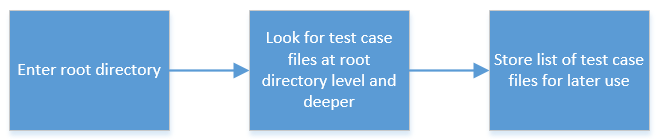
\includegraphics[width=0.75\textwidth]{./RecurDataFlow}
\end{center}
\caption{Recursive File Search Data Flow Diagram \label{DataFlowDiagram}}
\end{figure}



\subsection{Design Details}
\paragraph{}
This component uses the C++ library \textit{dirent.h} to access and traverse the root directory and its children. The root directory being the directory level from which the product is used. The algorithm looks for folders and then recursively calls its self on the path of found folders. This continues until no more children folders are found. Once this base case has been achieved the algorithm works its way out of the recursion by checking the folder it is in for files that are test cases and returns to the next higher directory level. 
\paragraph{}
The algorithm finds pairs of test case files, namely [filename].tst and [filename].ans. Once the algorithm is completed a check is done to ensure that each ".tst" file has a matching ".ans" file.


\section{Major Component: Iterative Executable Tester }
\begin{algorithm} [tbh]                     % enter the algorithm environment
\caption{Compile and test student programs}          % give the algorithm a caption
\label{alg2}                           % and a label for \ref{} commands later in the document
\begin{algorithmic}                    % enter the algorithmic environment
	\REQUIRE valid and compile-able .cpp source code
	\STATE Compile user specified source code
	\FOR {each test case}
	\STATE input test case (".tst") file to students program
	\STATE compare students output to test case answer (".ans")
	\IF {students output differs from test case answer}
		\STATE append student program failed to $"[source_code].log"$ file
	\ELSE
		\STATE append student program passed to $"[source_code].log"$ file
	\ENDIF
	\ENDFOR
\end{algorithmic}
\end{algorithm} 
\subsection{Technologies  Used}
Linux (Fedora 19, Ubuntu 13.1) Operating System: Used for basic runtime needs. G+ compiler: used to compile and run both our code and student code. For further information on these two system features, consult Linux documentation.
\subsection{Component  Overview}
This component is responsible for iteratively testing a student source code against multiple test cases.

\subsection{Phase Overview}
\begin{itemize}
\item[1.]
	Compile source code specified by the user.
\item[2.]
	Redirect input and output for student source code executable.
\item[3.]
	Input a test case into student source code executable.
\item[4.]
	Compare output of student source code executable to solution.
\item[5.]
	Record whether the student passed the test case or failed the test case.
\end{itemize}

\subsection{Data Flow Diagram}

\begin{figure} [tbh]
\begin{center}
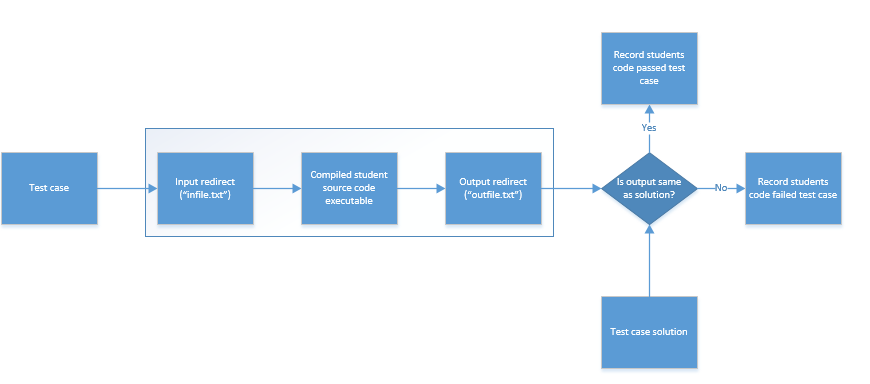
\includegraphics[width=1.0\textwidth]{./DataFlow}
\end{center}
\caption{Iterative Executable Tester Data Flow Diagram \label{DataFLowDiagram}}
\end{figure}

\paragraph{} The process illustrated in the figure above is repeated for all pairs of test cases found.


\subsection{Design Details}
\paragraph{}
This component implements \textit{popen} from \textit{stdlib.h}. This is used instead of a system call because it allows pipe-lining of the input and output for the system calls and effectively silences the student source code executable output to the command line. This provides a cleaner experience for the user.
\paragraph{}
When it is determined that a students source code either passed 
or failed a test case, it is recorded to [studentsourcecode].log.
 According to the customers requirements this file is not overwritten, instead the results of running the product are appended to the log file.